% Document class `report-template` accepts either project-plan or final-report option in
% []. This will change the title page as necessary.
\documentclass[project-plan]{report-template}
% \documentclass[final-report]{report-template}

% Packages I use in my report.
\usepackage{graphicx}
\usepackage{amsmath}
\usepackage{blindtext}

% Directory where I saved my figures.
\graphicspath{{./figures/}}

% Metadata used for the title page - please modify.
\university{Imperial College London}
\department{Department of Earth Science and Engineering}
\course{MSc in Applied Computational Science and Engineering}
\title{Computational modelling and simulation of a particle in vertical motion}
\author{Mickey Mouse}
\email{m.mouse@imperial.ac.uk}
\githubusername{acse-mm123}
\supervisors{Dr Bugs Bunny\\
             Prof. Donald Duck}
\repository{https://github.com/ese-msc-2023/irp-mm123}

\begin{document}

\maketitlepage  % generate title page

% Abstract
\section*{Abstract}
\blindtext  % outputs some dummy text

% Introduction section
\section{Introduction}
\blindtext[3]

% Another section
\section{Methods}
In this work, we wrote a simulation package for calculating the position of a particle in vertical motion as shown in Fig.~\ref{fig:experiment}. We compute the position $y(t)$ at time $t$ using:

% Equation
\begin{equation}
    \label{eq:vertical-position}
    y(t) = v_{0}t - \frac{1}{2}gt^{2},
\end{equation}

where $v_{0}$ is the initial velocity, and $g$ is the acceleration due to the Earth's gravity.

% Figure
\begin{figure}
    \begin{center}
        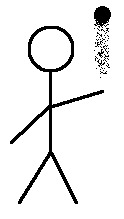
\includegraphics[width=0.2\textwidth]{experiment.jpg}
    \end{center}
    \caption{\label{fig:experiment} Particle in vertical motion.}
\end{figure}

Python code we implemented for computing $y(t)$ is:

% Code listing
\begin{lstlisting}[language=Python]
def position(t, v0=0, g=9.81):
    """Position of a particle in verticle motion."""
    return v0*t - 0.5*g*t**2
\end{lstlisting}

We made our computational workflows reproducible using Jupyter~\cite{Beg2021}.

\section{Results}
\blindtext[3]

\section{Discussion}
\blindtext[2]

\section{Conclusion}
\blindtext[2]

% References
\bibliographystyle{plain}
\bibliography{references}  % BibTeX references are saved in references.bib

\end{document}          
